\documentclass[12pt,a4paper]{article}
\usepackage[dutch]{babel}
\usepackage[utf8]{inputenc}
\usepackage[margin=0.5in]{geometry}
\usepackage{amsmath}
\usepackage{amsfonts}
\usepackage{amssymb}
\usepackage{graphicx}
\usepackage{listings}
\usepackage{float}
\usepackage{hyperref}



\begin{document}
\graphicspath{{images/}}
\DeclareGraphicsExtensions{.pdf,.png,.jpg}
\lstset{language=bash}
\author{Frank Willemsen}
\title{Een programma installeren met Synaptic}
\date{\today}
\maketitle
\abstract{Een beknopte Nederlandstalige inleiding tot het gebruik van Synaptic op Debian}
\section{Een programma installeren met Synaptic}


Je opent Synaptic. Dit programma vind je waarschijnlijk vinden onder Overige. Zo niet, dan kun je altijd \emph{Opdracht uitvoeren...} kiezen en dan "Synaptic" invoeren. 

\begin{figure} [H]
\centering
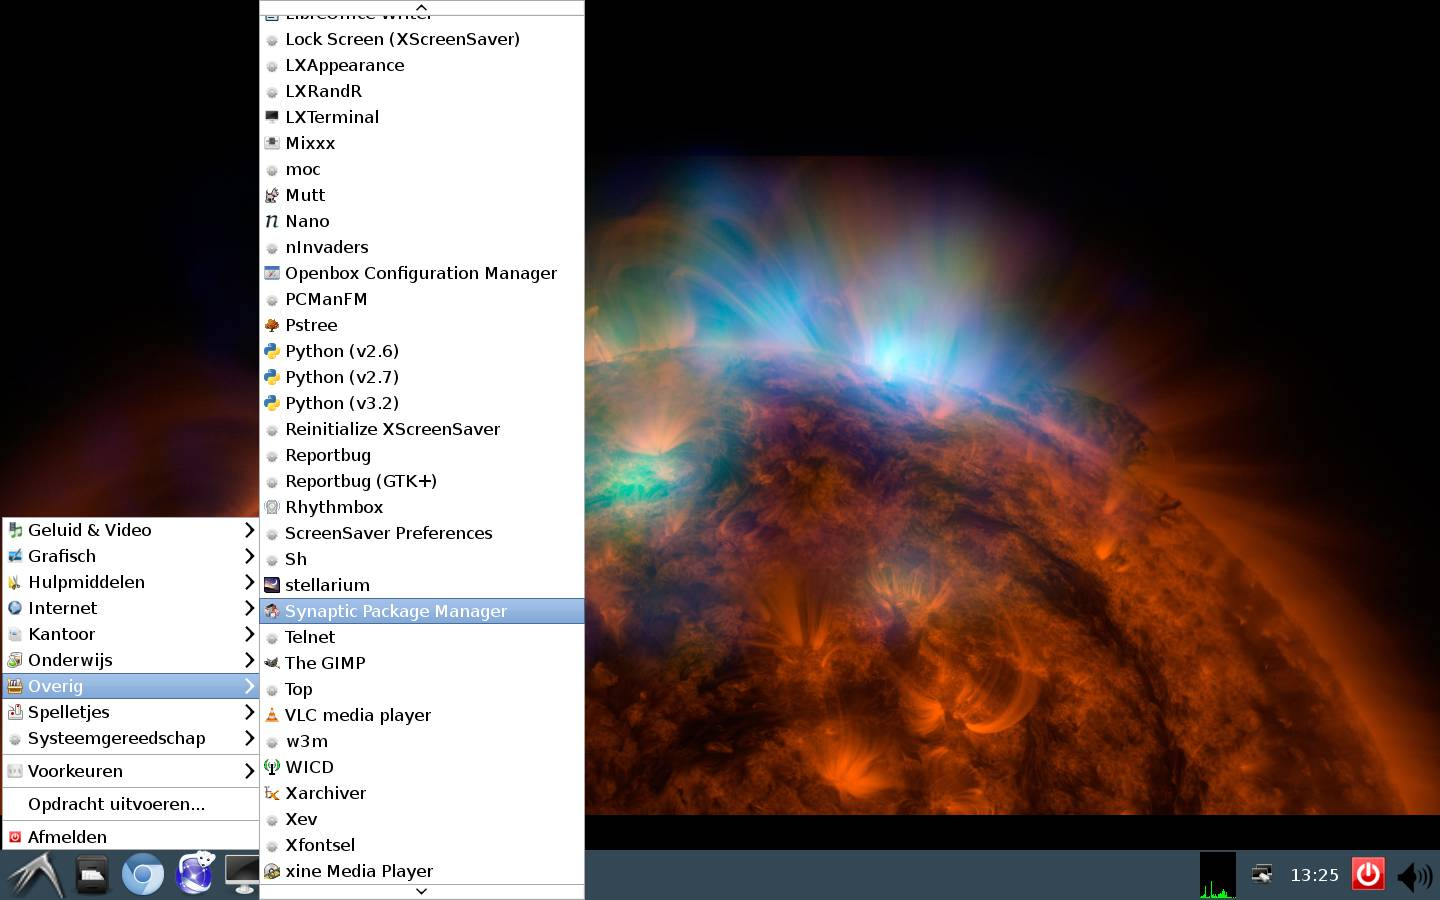
\includegraphics[width=0.45\textwidth]{plaatje01}
\caption{open Synaptic}
\label{plaatje01}
\end{figure}

Synaptic vraagt gelijk bij openen naar je wachtwoord. Het heeft dit nodig om software te kunnen te installeren of te verwijderen.

\begin{figure} [H]
\centering
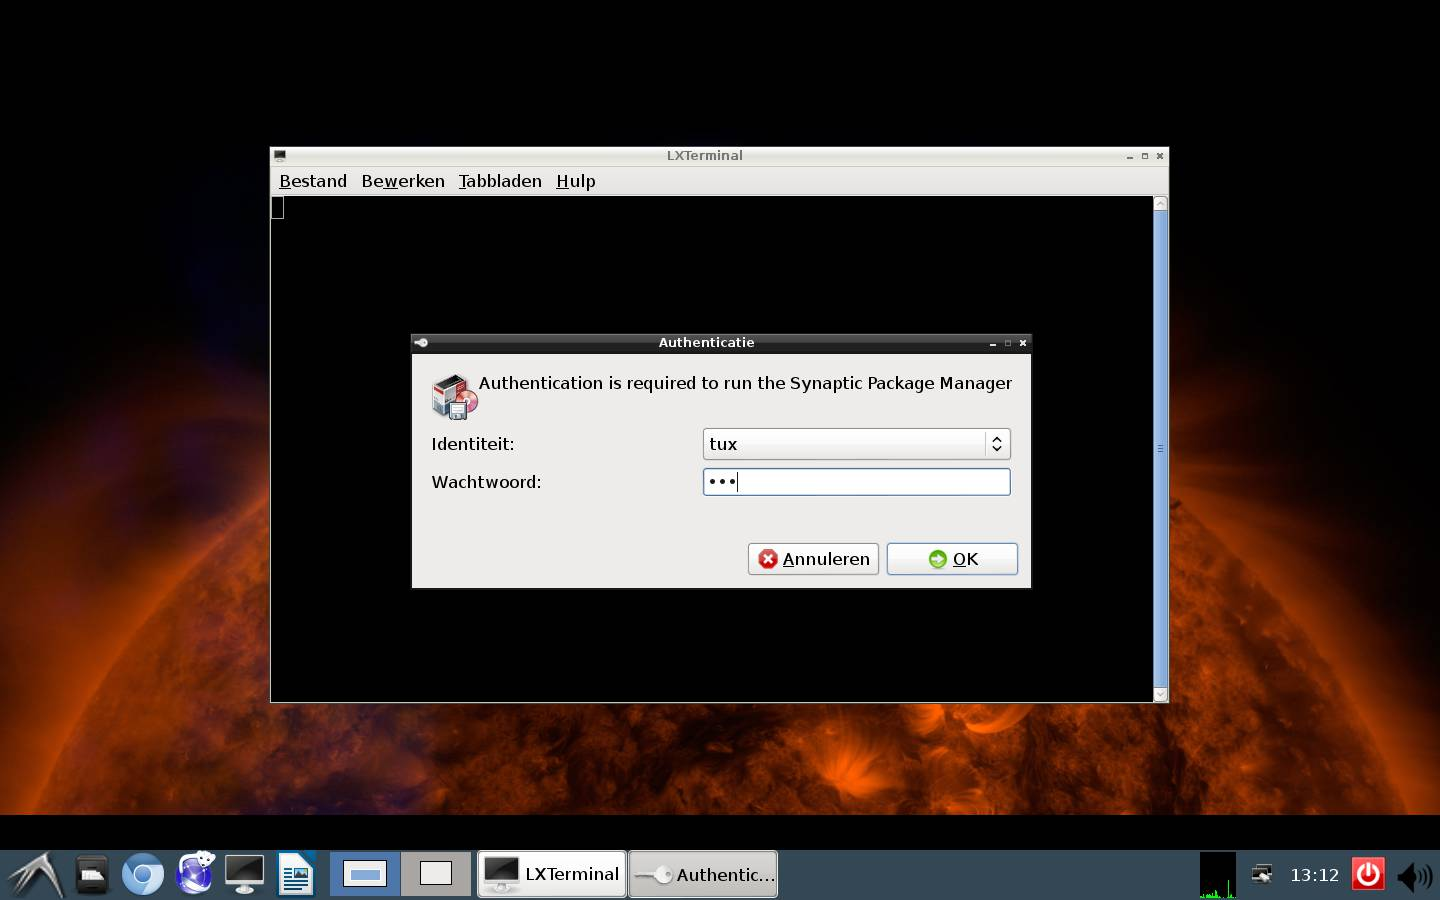
\includegraphics[width=0.45\textwidth]{plaatje02}
\caption{Wachtwoordinvoer}
\label{plaatje02}
\end{figure}

\clearpage

Nu je er toch bent, is het een goed idee om te herladen. Daarna weet je zeker dat je van alle programma's de nieuwste beschikbare versie kunt krijgen.

\begin{figure} [H]
\centering
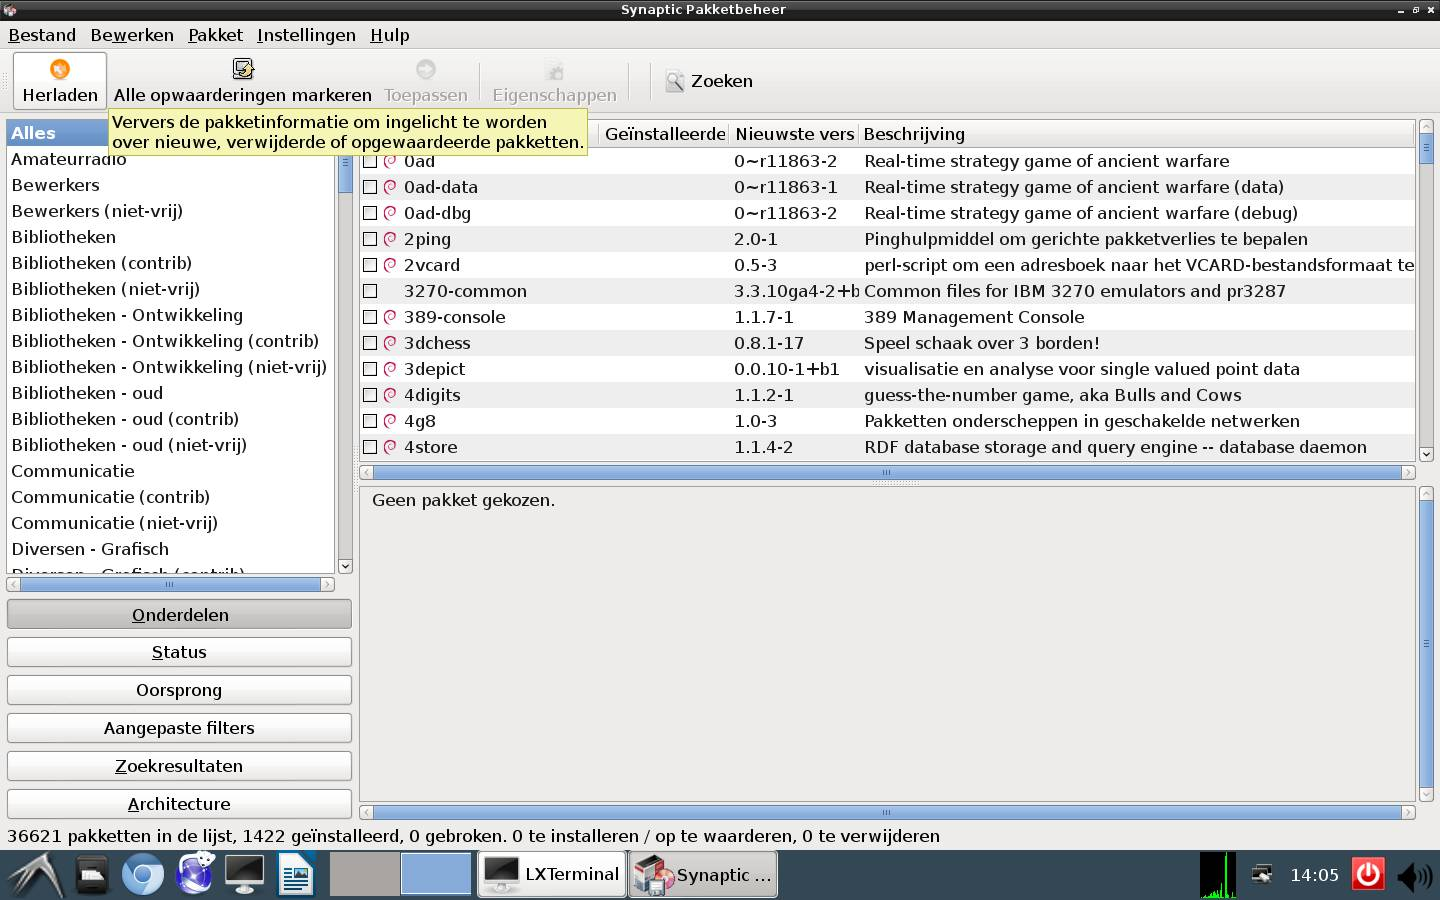
\includegraphics[width=0.45\textwidth]{plaatje04}
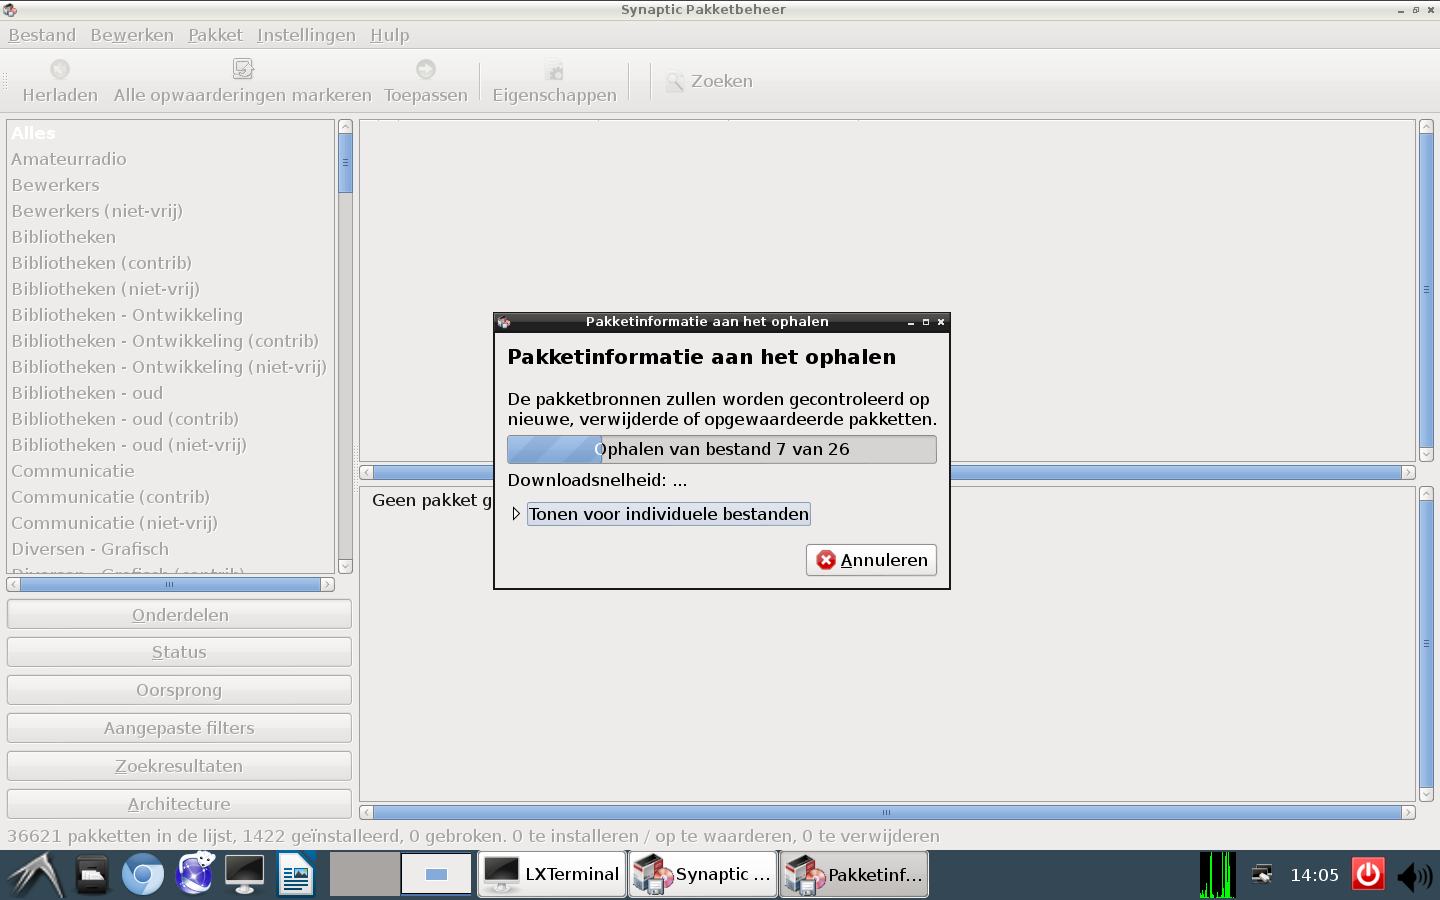
\includegraphics[width=0.45\textwidth]{plaatje05}
\caption{Pakketinformatie herladen}
\label{plaatje04}
\end{figure}

Als je weet welk programma je wilt installeren, hoef je niet moeilijk te doen en het in een menu op te zoeken. Je doet Zoeken en voert de naam in.

\begin{figure} [H]
\centering
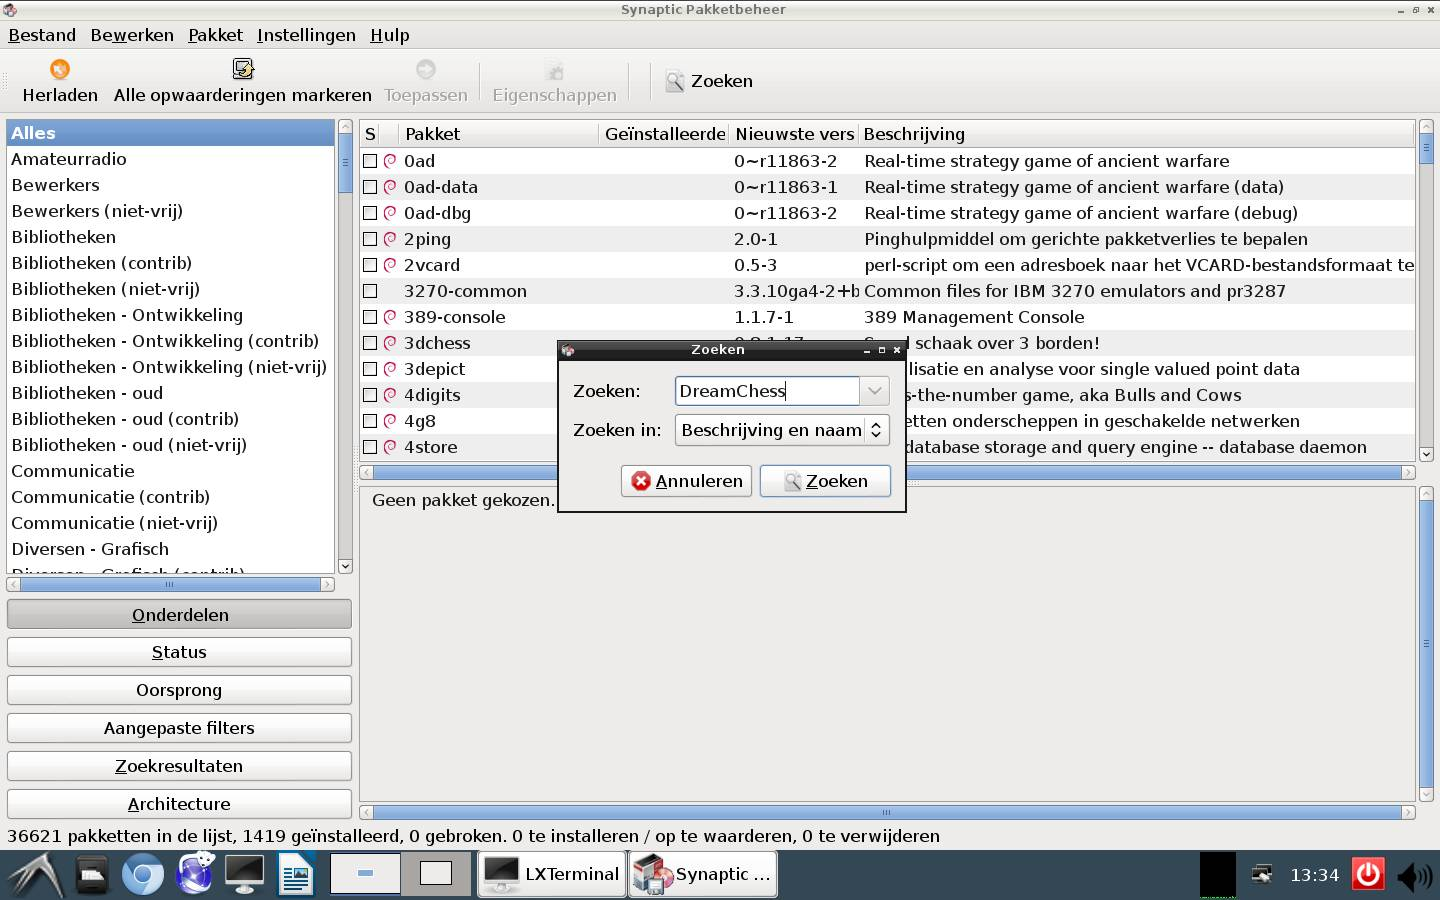
\includegraphics[width=0.45\textwidth]{plaatje06}
\caption{Zoeken naar een programma}
\label{plaatje06}
\end{figure}








\end{document}
